\chapter{Esiti Attività} % Main chapter title

\label{Capitolo6} % For referencing the chapter elsewhere, use \ref{Chapter1} 

\lhead{Capitolo 6. \emph{Esiti Attività}} % This is for the header on each page - perhaps a shortened title



\section{Esiti Analisi Statica}

Di seguito vengono riportati i risultati dell'analisi statica sul codice sorgente effettuata
con lo strumento JTest. Vengono riportati per ogni
classe:
\begin{itemize}


\item Classe: il nome della classe preceduto dall'indicazione del componente padre
\item CC: per la metrica di complessità ciclomatica viene riportato il valore ottenuto
dalla media aritmetica dei vari metodi di classe 
\item LOC: per la metrica di linee di codice viene riportato il valore intero ottenuto dalla
media aritmetica dei vari metodi di classe (per evitare di riportare i singoli
metodi)
\item LCOM HS:
il valore ottenuto dal calcolo della metrica LCOM HS che indica la
coesione dei metodi di una classe.

\end{itemize}

Il numero di campi dati e di metodi utilizzati per classe è una diretta fonte dei risultati ottenuti.


\begin{center}
    \begin{longtable}{ | p{6cm} | p{1.5cm} | p{1.5cm} | p{1.8cm} |}
    \hline
    Classe & CC & LOC & LCOM HS \\ \hline
    Activity::SplashScreenActivity& 1.2 & 5 & 0.15\\ \hline 
    Activity::FaceDetectionActivity& 3.33 & 15& 1.37\\ \hline 
    Activity::StaticFaceDetectionActivity& 1.81 & 12 & 0.8\\ \hline 
    Activity::PhotoActivity& 2.34 & 8 & 0.73\\ \hline 
    Activity::TutorialActivity& 2.55 & 4  & 0.42\\ \hline 
    Service::BootStartUpReceiver & 1 & 3 & 0.25\\ \hline 
    Service::BackgroundService & 1.33 & 5 & 0.25\\ \hline 
    Model::Data& 1.66 &  6  & 1.84\\ \hline 
    Model::Templates& 3.11 & 11  & 0\\ \hline 
    Model::Sprite& 1.82 & 5  & 0.51\\ \hline 
    Core::Camera& 1.2 & 12 & 0\\ \hline 
    Social::LoginSession& 2.73 & 5 & 0.15\\ \hline 
    Social::Share& 1.55 & 7 & 0\\ \hline 
    Utility::MatUtils& 1.27 & 5 & 0\\ \hline 
	Utility::Generics& 3.83 & 13 & 0\\ \hline 
	Adapter::CustomAdapter& 1.17 & 6 & 0.15\\ \hline     
    


    \end{longtable}
\end{center}

Complice la ridotta esperienza, durante lo sviluppo è stato necessario rivisitare ed affinare alcuni metodi per rientrare nel range di accettazione per la complessità ciclomatica scomponendo il problema in sotto-problemi di minore dimensioni e quindi più facilmente verificabili. A seguito di alcune controlli del codice tutti i limiti imposti sono stati rispettati.
Nella tabella a seguire sono presenti valori di \textit{LCOM HS} $=$ 0. Ciò possibile in quanto nella classe non sono presenti campi dati. Sono però presenti anche valori \textit{LCOM HS} > 1.0, che potrebbero indicare un campanello d'allarme. Nonostante sia difficile evitare tale problema, una migliore progettazione avrebbe potuto produrre valori di coesione migliori.


\section{Esiti Test di Validazione}

\begin{center}
    \begin{longtable}{ | p{2cm} | p{6cm} | p{2cm} | p{2cm} |}
    \hline
    Codice & Descrizione & Requisito & Esito \\ \hline
        & Verificato dal buon esito dei figli &RFO1 & \textcolor{green}{Positivo}\\ \hline 
    T1.1& Verificare il corretto funzionamento dell'attività e il caricamento dinamico dei parametri d'utilizzo in base al dispositivo utilizzato &RFO1.1 & \textcolor{green}{Positivo}\\ \hline 
    T1.2& Verificato dal buon esito dei figli  &RFO1.2 & \textcolor{green}{Positivo}\\ \hline 
    T1.2.1& Verificare la possibilità di cambiare camera a tempo d'esecuzione &RFO1.2.1 & \textcolor{green}{Positivo}\\ \hline 
    T1.2.2& Verifica la possibilità di cambiare l'elaborazione della camera (Nativa o Java) &RFO1.2.2 & \textcolor{green}{Positivo}\\ \hline 
   T1.2.3 &Verifica la possibilità di cambiare la risoluzione del frame in ingresso&RFO1.2.3 & \textcolor{green}{Positivo}\\ \hline 
    T1.2.4& Il test verifica la possibilità di cambiare il range operativo di campionamento &RFO1.2.4 & \textcolor{green}{Positivo}\\ \hline 
    T1.2.5&Il test verifica la possibilità di cambiare i parametri operativi di campiona-
mento &RFO1.2.5 & \textcolor{green}{Positivo}\\ \hline 
    T1.2.6&Il test verifica il corretto funzionamento di modifica delle parti da ricercare a
run-time &RFO1.2.6 & \textcolor{green}{Positivo}\\ \hline 
    T1.2.7&Il test verifica la possibilità di abilitare o disabilitare la modalità alto contrasto
e/o monocromatica &RFO1.2.7 & \textcolor{green}{Positivo}\\ \hline 
    T1.4& Verificato dal buon esito dei figli &RFD1.4 & \textcolor{green}{Positivo}\\ \hline 
    T1.4.1&Il test deve verificare il corretto caricamento degli Sprites &RFO1.4.1 & \textcolor{green}{Positivo}\\ \hline 
    T1.4.2&Il test deve verificare la corretta renderizzazione della ListView &RFO1.4.2 & \textcolor{green}{Positivo}\\ \hline 
    T1.4.3&Il test verifica verifica il corretto utilizzo dello Sprite assegnato &RFO1.4.3& \textcolor{green}{Positivo}\\ \hline 
    T2.1&Il test verifica il corretto caricamento di un'immagine dallo smartphone &RFO2.1  & \textcolor{green}{Positivo}\\ \hline 
    T3& Verificato dal buon esito dei figli &RFO3 & \textcolor{green}{Positivo}\\ \hline 
    T3.1& Il test verifica la possibilità di ridimensionare la foto scattata &RFD3.1 & \textcolor{green}{Positivo}\\ \hline 
    T3.2& Verificato dal buon esito dei figli &RFD3.2  & \textcolor{green}{Positivo}\\ \hline 
    T3.2.1&Il test verifica il caricamento della lista di applicazioni attraverso le quali
`e possibile condividere il contenuto &RFD3.2.1  & \textcolor{green}{Positivo}\\ \hline 
    T3.2.2&Il test verifica l'esito della condivisione&RFD3.2.2  & \textcolor{green}{Positivo}\\ \hline 
    T3.3& Verificato dal buon esito dei figli &RFD3.3  & \textcolor{green}{Positivo}\\ \hline 
    T3.3.1& Il test verifica la possibilità di eseguire il Login sulla piattaforma Facebook &RFD3.3.1  & \textcolor{green}{Positivo}\\ \hline 
    T3.3.2&Il test verifica il mantenimento della sessione successivo alla chiusura
dell'applicazione &RFD3.3.1  & \textcolor{green}{Positivo}\\ \hline 
    T3.3.3& Il test verifica l'integrità dei dati allegati alla foto, inseriti dall'utente &RFD3.3.2  & \textcolor{green}{Positivo}\\ \hline 
    T3.3.4& Il test verifica il caricamento e l'esito della condivisione&RFD3.3.3  & \textcolor{green}{Positivo}\\ \hline 
    \end{longtable}
\end{center}


\section{Analisi Prestazionale}

Al fine di verificare le prestazioni ottenute in media dall'applicativo, l'azienda ha fornito 4 dispositivi che rappresentano all'anno della stesura di questo documento (2014) le possibili fasce di mercato.

I dispositivi forniti sono:

\begin{itemize}
\item \textbf{Fascia Alta - \textit{Galaxy S4}} 
	\begin{itemize}
		\item CPU quad core 1.6GHz Cortex A15 
		\item RAM 2 GB 
		\item Fotocamera : posteriore: 13 MP , anteriore 2.1 MP
		\item Android 4.2.2 Jelly Bean 
	\end{itemize}
\item \textbf{Fascia Media - \textit{Galaxy S3 Mini}}
	\begin{itemize}
		\item CPU 1 GHz dual core ARM Cortex A9
		\item RAM 1 GB 
		\item Fotocamera : posteriore: 5 MP , anteriore 1.3 MP
		\item Android 4.1.1 Jelly Bean 
	\end{itemize}
\item \textbf{Fascia Bassa - \textit{Galaxy Fame}}
	\begin{itemize}
		\item CPU 0.85 GHz single core ARM Cortex A9
		\item RAM 512 MB
		\item Fotocamera : posteriore: 3 MP , anteriore 1.3 MP
		\item Android 2.3.0 Gingerbread
	\end{itemize}
\end{itemize}

Dal momento che le prestazioni possono dipendere dalla qualità della luce e dalla distanza dell utente dal dispositivo, si è preferito testare l'applicazione utilizzando video come input. Le variabili tenute in considerazione sono risoluzione, numero di volti, numero di falsi positivi, numero di fotogrammi medi per secondo al termine di ogni video. I video sono sono volutamente caratterizzati da camere mobili, e da scene in cui non sono presenti persone al fine di verificare la presenza di falsi positivi.

I video utilizzati sono reperibili direttamente dal web ai link:

\begin{itemize}
\item[•] \href{http://www.youtube.com/watch?v=XFTbN10f_Fg}{Video 1 : Matrix - The red Woman}
\item[•] \href{http://www.youtube.com/watch?v=yWPyRSURYFQ}{Video 2 : Blade Runner - She's a Replicant}
\item[•] \href{http://www.youtube.com/watch?v=s3rv0BdxWfM}{Video 3 : The Heat - The Sun Rises and Sets With Her }
\end{itemize}

Risoluzioni utilizzate:

\begin{itemize}
\item[•] $1280\ast720$ 
\item[•] $640\ast480$ 
\item[•] $320\ast240$ 
\end{itemize}

I test sono stati effettuati con i seguenti parametri precedentemente definiti in sezione:
\begin{itemize}
\item \textit{FaceDetectionActivity::minNeighbors} = 3 (sono necessari almeno 3 hit per frame per confermare positivamente il volto)
\item \textit{FaceDetectionActivity::minSize} = -1  
\item \textit{FaceDetectionActivity::maxSize} = -1
\item \textit{FaceDetectionActivity::scaleFactor} = 1.1 
\end{itemize}

In questo modo ci si assicura che il costo computazionale per ogni frame sia massimo (il metodo di rilevamento facciale terminerà solo dopo aver valutato l'immagine nella sua interezza). 
Dato che per ogni singolo frame vi possono essere più hits corrispondenti allo stesso volto, è stata creata una semplice funzione ad hoc che permetta di contare un solo volto per set coincidenti di hits. Inoltre tali video sono stati velocizzati aumentando il framerate (24$\longmapsto$ 72 fotogrammi per secondo) per evitare qualsiasi problema di Input bound.


\begin{figure}[h]\centering  
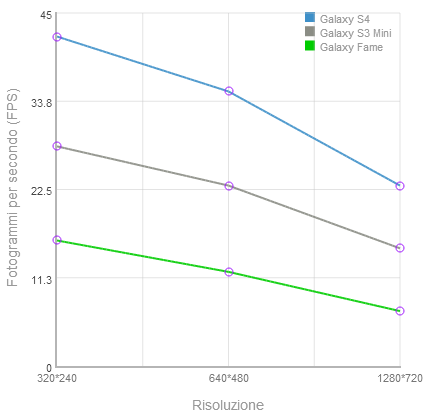
\includegraphics[scale=0.6]{/home/nicgen/Scrivania/thesis/Figures/fps.png}
\caption[Grafico prestazionale riassuntivo]{Graifco prestazionale riassuntivo}
\label{pic-a}
\end{figure}

Come previsto, al variare dei dispositivi non vi è alcuna differenza nei risultati (quantità di volti rilevati + $\varepsilon$(falsi positivi rilevati)) se non al variare del parametro \textit{FaceDetectionActivity::MinNeighbors}. Infatti,prendendo come risoluzione di riferimento $640 \ast 480$, sono stati ottenuti i seguenti risultati
\\
GRAFICO A RES FISSA CON NUM FALSI POSITIVI E NEGATIVI AL VARIARE DELLA RETENTION 
\\
I risultati sono però stati totalmente differenti nell'utilizzo reale utilizzando la fotocamera posteriore come input al posto dei video (che garantivano un framerate costante di 72 fotogrammi per secondo). 
\\
GRAFICO LUMINOSITA NORMALE

GRAFICO LUMINOSITA BASSA
\\
Infine si può notare come vi siano grosse discrepanze di prestazioni al variare della fotocamera d'input (Anteriore o Posteriore). Questo è dovuto al fatto che generalmente la fotocamera posteriore è di qualità maggiore (sensore di dimensioni maggiori, diaframma più aperto ed ISO che può raggiungere valori più elevati)
\\
GRAFICO FRONTALE VS POSTERIORE

\subsection{Considerazioni}

A seguito dei test effettuati l'idea è che i dispositivi correntemente presenti sul mercato abbiamo una potenza computazionale più che sufficiente per eseguire tali task con prestazioni discrete e garantiscano un'esperienza d'utilizzo adeguata. Il maggior problema riscontrato è sicuramente la qualità della fotocamera che può condizionare drasticamente le performance se posta in condizione d'utilizzo non ottimale. Il software preinstallato sullo smartphone infatti, in condizioni di bassa luminosità, tende ad alzare il valore ISO (sensibilità del sensore) ed ad utilizzare un diaframma il più aperto possibile. La necessità di miniaturizzare l'hardware fotografico ha però come conseguenza quella di non poter avere sensori e lenti di dimensioni adeguate. Questo si traduce in bassa qualità, e pertanto per ogni singolo frame di un video sarà necessario un tempo di esposizione molto elevato. Lo stream di fotogrammi risulterà quindi caratterizzato da un framerate molto basso, ponendo il processore in attesa attiva del fotogramma da processare. 

